\documentclass[a4paper,12pt]{article}
\usepackage{tabularx}
\usepackage{amsmath}
\usepackage[utf8]{inputenc}
\usepackage{multicol}
\usepackage{cancel}
\usepackage{amsmath, amssymb, amsthm}
\usepackage{graphicx}
\usepackage{enumitem}
\usepackage{array}
\usepackage[left=2cm, right=2cm, top=2cm, bottom=2cm]{geometry}
\usepackage{fancyhdr}
\usepackage{xfp}
\usepackage{pgf}
\usepackage{tikz}

\usepackage{graphicx}
\usepackage{fancyhdr}

\setlength{\headheight}{28pt} % genug Platz für das Logo
\pagestyle{fancy}
\fancyhf{} % alles leeren
\fancyhead[L]{\includegraphics[height=1.2cm]{logo.png}}
\fancyhead[C]{\small Klassenarbeit – Rechnen mit Potenzen \ (Kl. G9A)}
\fancyhead[R]{\small Name:\ \rule{2.8cm}{0.4pt}}
\fancyfoot[C]{\thepage}

\fancyfoot[C]{Seite \thepage \enspace\textbullet\enspace J.\,Mycan \textcopyright~2025 *Klassenarbeit 45 min.*}

\renewcommand{\footrulewidth}{0.4pt}

%\pagestyle{fancy}
%\lhead{Klassenarbeit 45min.}
%\chead{Heinrich-von-Kleist-Schule}
%\rhead{Mathematik - G8A}
%\lfoot{}
%\cfoot{Seite \thepage}
%\rfoot{}

\newcommand{\punkteA}{8}
\newcommand{\punkteB}{6}
\newcommand{\punkteC}{6}
\newcommand{\punkteD}{18}
\newcommand{\punkteE}{6}
%\newcommand{\punkteF}{12}

\newcommand{\maxSumme}{42}
\newcommand{\noteEinsMin}{\fpeval{round(\maxSumme * 0.95,0)}}
\newcommand{\noteZweiMin}{\fpeval{round(\maxSumme * 0.80,0)}}
\newcommand{\noteDreiMin}{\fpeval{round(\maxSumme * 0.60,0)}}
\newcommand{\noteVierMin}{\fpeval{round(\maxSumme * 0.45,0)}}
\newcommand{\noteFunfMin}{\fpeval{round(\maxSumme * 0.20,0)}}
\newcommand{\noteSechsMin}{0}

\newcommand{\summe}{%
	\pgfmathparse{\punkteA + \punkteB + \punkteC + \punkteD + \punkteE}%
	\pgfmathprintnumber{\pgfmathresult}}

\begin{document}
	
%	\begin{center}
%		\textbf{Klassenarbeit - Lineare Funktionen und LGS}
%	\end{center}
	
%	\textbf{Vor- und Nachname:} \underline{\hspace{10cm}}\\[0.1cm]
%\vspace{2cm}
	
%	\textbf{Vor- und Nachname:} \underline{\hspace{10cm}}\\[0.1cm]
%Die Lösungen sowie Lösungswege sollten klar strukturiert und gut nachvollziehbar sein. \\[0.1cm]
		% -------------------------------------------------
	% Aufgabe 1
	% -------------------------------------------------
	\textbf{Aufgabe 1 (8 Punkte)}\\
	Im folgenden Koordinatensystem sind vier verschiedene Parabeln eingezeichnet:
	\begin{center}
		\begin{minipage}{0.55\textwidth}
			\centering
			\begin{tikzpicture}[scale=0.9]
				% Koordinatensystem [-4,4] x [-4,4] mit Gitter
				\draw[step=1,very thin,gray!40] (-4,-4) grid (4,4);
				\draw[->] (-4,0) -- (4.3,0) node[right] {$x$};
				\draw[->] (0,-4) -- (0,4.3) node[above] {$y$};
				
				% Achsenbeschriftung
				\foreach \x in {-3,-2,-1,1,2,3}
				\draw (\x,0.1) -- (\x,-0.1) node[below=2pt] {\scriptsize \x};
				\foreach \y in {-3,-2,-1,1,2,3}
				\draw (0.1,\y) -- (-0.1,\y) node[left=2pt] {\scriptsize \y};
				
				% Graph I: f(x) = 1/4 x^2 - 2 (nach oben geöffnet, leicht nach unten verschoben)
				\draw[thick,domain=-4:4,smooth,variable=\x]
				plot ({\x},{0.25*\x*\x - 2});
				\node[font=\small] at (0,-2.4) {\textbf{I}};
				
				% Graph II: f(x) = 3/4 (x-1)^2 - 3 (nach oben, nach rechts/unten verschoben)
				\draw[thick,dashed,domain=-2:4,smooth,variable=\x]
				plot ({\x},{0.75*(\x-1)*(\x-1) - 3});
				\node[font=\small] at (1,-3.4) {\textbf{II}};
				
				% Graph III: f(x) = -1/4 x^2 + 3 (nach unten, nach oben verschoben)
				\draw[thick,dotted,domain=-4:4,smooth,variable=\x]
				plot ({\x},{-0.25*\x*\x + 3});
				\node[font=\small] at (0,3.4) {\textbf{III}};
				
				% Graph IV: f(x) = -3/4 (x+1)^2 + 3 (nach unten, nach links/oben verschoben)
				\draw[thick,densely dashed,domain=-4:2,smooth,variable=\x]
				plot ({\x},{-0.75*(\x+1)*(\x+1) + 3});
				\node[font=\small] at (-1,3.4) {\textbf{IV}};
				
			\end{tikzpicture}
		\end{minipage}%
		\hfill
		\begin{minipage}{0.4\textwidth}
			\small
			\textbf{Zuordnung:}\\[0.5em]
			Ordne jedem Graphen \textbf{I–IV} genau eine der folgenden
			Funktionsgleichungen zu.
			
			\begin{align*}
				\text{A)}\quad & f(x) = \tfrac{1}{4}x^{2} - 2 \\
				\text{B)}\quad & f(x) = \tfrac{3}{4}(x-1)^{2} - 3 \\
				\text{C)}\quad & f(x) = -\tfrac{1}{4}x^{2} + 3 \\
				\text{D)}\quad & f(x) = -\tfrac{3}{4}(x+1)^{2} + 3 \\
				\text{E)}\quad & f(x) = \tfrac{1}{2}x^{2} + 1
			\end{align*}
		\end{minipage}
	\end{center}
	
	Im Koordinatensystem sind vier Parabeln mit folgenden Gleichungen eingezeichnet:

	Die Zuordnung ist:
	
	\[
	\boxed{
		\text{I} \leftrightarrow \text{A},\quad
		\text{II} \leftrightarrow \text{B},\quad
		\text{III} \leftrightarrow \text{C},\quad
		\text{IV} \leftrightarrow \text{D}
	}
	\]
	Die Funktionsgleichung E passt zu keinem der eingezeichneten Graphen.
	
	\medskip
	\textbf{Begründung in Schritten:}
	\begin{itemize}
		\item Graph I ist nach oben geöffnet und hat den Scheitelpunkt bei \(S(0\mid -2)\).  
		Das passt genau zu \(f(x) = \tfrac{1}{4}x^{2}-2\) (Scheitel bei \((0\mid -2)\)).
		\item Graph II ist nach oben geöffnet, nach rechts verschoben (Scheitel bei \(x=1\)) 
		und nach unten verschoben.  
		Das passt zu \(f(x) = \tfrac{3}{4}(x-1)^{2}-3\).
		\item Graph III ist nach unten geöffnet, kein \(x\)-Verschiebung und Scheitel bei 
		\((0\mid 3)\).  
		Das passt zu \(f(x) = -\tfrac{1}{4}x^{2}+3\).
		\item Graph IV ist nach unten geöffnet, nach links verschoben (Scheitel bei \(x=-1\))
		und nach oben verschoben (Scheitelhöhe \(y=3\)).  
		Das passt zu \(f(x) = -\tfrac{3}{4}(x+1)^{2}+3\).
		\item Die Funktionsgleichung E \(f(x)=\tfrac{1}{2}x^{2}+1\) ist eine nach oben
		geöffnete Parabel mit Scheitel bei \((0\mid 1)\); eine solche Parabel ist im Bild nicht vorhanden.
	\end{itemize}
	\newpage
	% -------------------------------------------------
	% Aufgabe 2
	% -------------------------------------------------
\textbf{Aufgabe 2 (Punkte)}\\
	Bringe die folgenden quadratischen Funktionen jeweils in die \emph{Scheitelpunktform}.
	
\begin{enumerate}
	\item[a)] Gegeben ist der Scheitelpunkt der Normalparabel \(S(-2\mid 3)\).
	
	\item[b)] Gegeben ist die quadratische Funktion \(f(x) = -1{,}5x^{2} - 12x + 18\).
	
	\item[c)] Eine quadratische Funktion \(g\) besitzt die Nullstellen \(x_1 = -1\)
	und \(x_2 = 6\) und hat den Streckfaktor \(a = 2\).
\end{enumerate}

\textbf{Lösung zu Aufgabe 2}\\[0.5em]
\begin{enumerate}
	\item[a)] Scheitelpunktform hat allgemein die Form \(y=a(x-x_S)^2+y_S\).
	Bei der Normalparabel gilt \(a=1\) und \(S(-2\mid 3)\).
	\[
	f(x)=(x-(-2))^2+3=(x+2)^2+3.
	\]
	\[
	\boxed{f(x)=(x+2)^2+3}
	\]
	
	\item[b)] Gegeben:
	\[
	f(x)=-1{,}5x^2-12x+18.
	\]
	Faktor \(-1{,}5\) aus den ersten beiden Termen ausklammern:
	\[
	f(x)=-1{,}5\bigl(x^2+8x\bigr)+18.
	\]
	Quadratische Ergänzung: \(x^2+8x=(x+4)^2-16\).
	\[
	f(x)=-1{,}5\bigl((x+4)^2-16\bigr)+18
	=-1{,}5(x+4)^2+24+18
	=-1{,}5(x+4)^2+42.
	\]
	\[
	\boxed{f(x)=-1{,}5(x+4)^2+42}
	\]
	
	\item[c)] Nullstellenform mit \(x_1=-1,\;x_2=5,\;a=2\):
	\[
	g(x)=2(x-(-1))(x-5)=2(x+1)(x-5).
	\]
	Scheitel-x ist die Mitte der Nullstellen:
	\[
	x_S=\frac{-1+5}{2}=2.
	\]
	Scheitel-y durch Einsetzen:
	\[
	g(2)=2(2+1)(2-5)=2\cdot 3\cdot(-3)=-18.
	\]
	Also Scheitelpunktform:
	\[
	g(x)=2(x-2)^2-18.
	\]
	\[
	\boxed{g(x)=2(x-2)^2-18}
	\]
\end{enumerate}
\newpage	
	% -------------------------------------------------
	% Aufgabe 3
	% -------------------------------------------------
\textbf{Aufgabe 3 (9 Punkte)}\\[0.3em]
Die Skizze rechts zeigt den Korbwurf eines Basketballspielers.\\
a) Welche der folgenden Funktionen gibt die dargestellte Flugbahn wieder?
Begründe \underline{\textbf{kurz}} deine Antwort.\\

\noindent
\begin{minipage}[t]{0.45\textwidth}
	\vspace{0pt}
	
	\[
	\begin{aligned}
		f(x) &= -2x^{2} + 12x - 14\\[2pt]
		g(x) &= 2x^{2} + 12x - 13\\[2pt]
		h(x) &= -2(x-4)^2 -1
	\end{aligned}
	\]
	
	
	\medskip
	b) Der Ball verließ die Hand des Spielers beim \(x\)-Wert \(2\). Wie hoch war die Hand beim Abwurf?\\[0.6em]
	c) Berechne den höchsten Punkt der Flugbahn des Balles.
\end{minipage}%
\hfill
\begin{minipage}[t]{0.40\textwidth}
	\vspace{0pt}
	\centering
	\includegraphics[width=\textwidth]{baskettball.png}
\end{minipage}

\textbf{Lösung zu Aufgabe 3}\\[0.5em]
\textit{Wie vorgegeben wird für die Rechnungen die Funktion \textbf{A} (erste Funktion) verwendet:}
\[
A(x)=f(x)=-2x^{2}+12x-14.
\]

\begin{enumerate}
	\item[a)] \textbf{Kurze Begründung (passender Graph).}\\
	Eine Flugbahn ist eine nach unten geöffnete Parabel \(\Rightarrow a<0\).
	\[
	f(x)=-2x^2+12x-14 \;\Rightarrow\; a=-2<0 \quad (\text{passt})
	\]
	\[
	g(x)=2x^2+12x-13 \;\Rightarrow\; a=2>0 \quad (\text{öffnet nach oben, passt nicht})
	\]
	\[
	h(x)=-2(x-4)^2-1 \;\Rightarrow\; \text{Scheitel }(4,-1)\ (\text{liegt unterhalb, passt nicht zur Skizze})
	\]
	Daher passt \(\boxed{f}\).
	
	\item[b)] \textbf{Abwurfhöhe bei \(x=2\) (mit Funktion A).}
	\[
	f(2)=-2\cdot 2^2+12\cdot 2-14=-2\cdot 4+24-14=-8+24-14=2.
	\]
	\[
	\boxed{\text{Die Abwurfhöhe beträgt } 2\,\text{m}.}
	\]
	
	\item[c)] \textbf{Höchster Punkt (Scheitelpunkt) (mit Funktion A).}\\
	Für \(ax^2+bx+c\) gilt \(x_S=-\frac{b}{2a}\).
	\[
	a=-2,\ b=12 \quad\Rightarrow\quad x_S=-\frac{12}{2\cdot(-2)}=-\frac{12}{-4}=3.
	\]
	\[
	y_S=f(3)=-2\cdot 3^2+12\cdot 3-14=-2\cdot 9+36-14=-18+36-14=4.
	\]
	\[
	\boxed{\text{Höchster Punkt: } S(3\mid 4)\ \text{(maximale Höhe }4\,\text{m}).}
	\]
\end{enumerate}


\newpage
	% -------------------------------------------------
	% Aufgabe 4
	% -------------------------------------------------
	\textbf{Aufgabe 4 (12 Punkte)}\\
	Löse folgende quadratische Gleichungen:
	
	\begin{enumerate}
		\item[a)] \(2x^{2} - 3x = x^{2} - x\)
		
		\item[b)] \((x + 1)^{2} + 2x = 2x^{2} - 3\)
		
		\item[c)] \(3(x - 2)^{2} + 2x = 2x^{2} + 5(x - 1) - 4\)
	\end{enumerate}

\textbf{Lösung zu Aufgabe 4}\\[0.5em]
\begin{enumerate}
	\item[a)] \(3x^{2} - 7x = x^{2} - x\)
	\[
	3x^2-7x-(x^2-x)=0
	\;\Rightarrow\; 2x^2-6x=0
	\;\Rightarrow\; 2x(x-3)=0
	\]
	\[
	\Rightarrow\; x=0 \;\text{ oder }\; x=3.
	\]
	\[
	\boxed{\mathcal{L}=\{0,3\}}
	\]
	
	\item[b)] \((x + 1)^{2} + 2x = 2x^{2} + 4\)
	\[
	(x+1)^2+2x = x^2+2x+1+2x = x^2+4x+1
	\]
	\[
	x^2+4x+1 = 2x^2+4
	\;\Rightarrow\; 0 = 2x^2+4-(x^2+4x+1)
	\;\Rightarrow\; x^2-4x+3=0
	\]
	\[
	x^2-4x+3=(x-1)(x-3)=0
	\;\Rightarrow\; x=1 \;\text{ oder }\; x=3.
	\]
	\[
	\boxed{\mathcal{L}=\{1,3\}}
	\]
	
	\item[c)] \(3(x - 2)^{2} + 2x = 2x^{2} + 5(x - 1) - 19\)
	\[
	3(x-2)^2+2x = 3(x^2-4x+4)+2x = 3x^2-12x+12+2x = 3x^2-10x+12
	\]
	\[
	2x^2 + 5(x-1) - 19 = 2x^2 + 5x - 5 - 19 = 2x^2+5x-24
	\]
	\[
	3x^2-10x+12 = 2x^2+5x-24
	\;\Rightarrow\; x^2-15x+36=0
	\]
	\[
	x^2-15x+36=(x-3)(x-12)=0
	\;\Rightarrow\; x=3 \;\text{ oder }\; x=12.
	\]
	\[
	\boxed{\mathcal{L}=\{3,12\}}
	\]
\end{enumerate}

\newpage
	% -------------------------------------------------
	% Aufgabe 5
	% -------------------------------------------------
	\textbf{Aufgabe 5 (Punkte)}\\
Ein Landwirt will an einer geraden Mauer einen rechteckigen Hühnerhof mit
Maschendraht abgrenzen. Die Mauer bildet dabei \emph{eine} Seite des
Rechtecks, für die keine Einzäunung benötigt wird. Es stehen insgesamt
\(20\,\text{m}\) Maschendraht zur Verfügung.

\medskip
Wie groß müssen die Seitenlängen des Rechtecks gewählt werden, damit die
Hühner möglichst viel Platz haben? Begründe dein Ergebnis.

\begin{center}
	\begin{minipage}[t]{0.45\textwidth}
		\centering
		% ggf. kleine Skizze des Rechtecks an der Mauer
		\includegraphics[width=\textwidth]{hof.png}
	\end{minipage}
\end{center}

\textbf{Lösung zu Aufgabe 5}\\[0.5em]
Sei \(x\) die Länge der beiden Seiten \emph{senkrecht} zur Mauer und \(y\) die Länge der Seite \emph{parallel} zur Mauer (gegenüber der Mauer).

\medskip
\textit{1) Zaunbedingung aufstellen}\\
Es müssen nur drei Seiten eingezäunt werden:
\[
2x + y = 20 \quad\Rightarrow\quad y = 20 - 2x.
\]

\medskip
\textit{2) Flächenfunktion aufstellen}\\
Die Fläche des Rechtecks ist
\[
A = x\cdot y \quad\Rightarrow\quad A(x)=x(20-2x)=20x-2x^2.
\]

\medskip
\textit{3) Maximum bestimmen}\\
\[
A(x)=-2x^2+20x
\]
ist eine nach unten geöffnete Parabel, also liegt das Maximum im Scheitel.
\[
x_S=-\frac{b}{2a}=-\frac{20}{2\cdot(-2)}=5.
\]
Dann
\[
y=20-2\cdot 5=10.
\]

\medskip
\textit{4) Maximaler Flächeninhalt (Kontrolle)}\\
\[
A_{\max}=5\cdot 10=50\ \text{m}^2.
\]

\textbf{Antwort:}\;
Die Seiten müssen \(\boxed{x=5\,\text{m}}\) (zweimal) und \(\boxed{y=10\,\text{m}}\) sein.
Dann ist der maximale Flächeninhalt \(\boxed{50\,\text{m}^2}\).


	
\end{document}
